\special{! TeXDict begin /landplus90{true}store end }

\documentclass[xga]{xdvislides}
\usepackage[landscape]{geometry}
\usepackage{graphics}
\usepackage{graphicx}
\usepackage{colordvi}
\usepackage[normalem]{ulem}

\newcommand{\smallish}{\fontsize{16}{16}\selectfont}

\begin{document}
\setfontphv

%%% Headers and footers
\lhead{\slidetitle}                               % default:\lhead{\slidetitle}
\chead{CS765 - Aspects of System Administration}% default:\chead{\relax}
\rhead{Slide \thepage}                       % default:\rhead{\sectiontitle}
\lfoot{\Gray{System Security}}% default:\lfoot{\slideauthor}
\cfoot{\relax}                               % default:\cfoot{\relax}
\rfoot{\Gray{\today}}
\vspace*{\fill}
\begin{center}
	\Hugesize
		CS615 - Aspects of System Administration\\ [1em]
		System Security\\ [1em]
	\hspace*{5mm}\blueline\\ [1em]
	\Normalsize
		Department of Computer Science\\
		Stevens Institute of Technology\\
		Jan Schaumann\\
		\verb+jschauma@stevens.edu+ \\
		\verb+https://www.cs.stevens.edu/~jschauma/615/+
\end{center}
\vspace*{\fill}

\subsection{This lecture}
What I won't tell you:
\begin{itemize}
	\item How to make your system "secure".
	\item How to break into other systems.
	\item Everything you need to know.
\end{itemize}
\vspace{.5in}
What I will tell you:
\begin{itemize}
	\item What you need to know to {\em start looking}.
	\item What concepts are critical to understand.
	\item What conceptual pitfalls you are likely to encounter.
	\item A few {\em always} and {\em never}s.
\end{itemize}


\subsection{Where/how does 'security' come into play?}

\subsection{Where/how does 'security' come into play?}
Lecture 02 (Filesystems, Disks, Storage)
\begin{itemize}
	\item storage model (DAS, NAS, SAN, Cloud)
	\item partitions / mount options
	\item filesystem features (permissions, access control lists)
	\item DoS on disk space
	\item firmware compromise on hard drives
\end{itemize}
\vspace{.5in}
Lecture 03 (Software Installation Concepts)
\begin{itemize}
	\item software package management and updates
	\item VMs, containers, etc.
	\item patch management
	\item package integrity checking
\end{itemize}

\subsection{Where/how does 'security' come into play?}
Lecture 04 (Multiuser Fundamentals)
\begin{itemize}
	\item privileges and trust models
	\item authentication methods, multi-factor authentication
	\item file access controls
	\item raising privileges
\end{itemize}
\vspace{.5in}
Lecture 05 / 06 (Networking)
\begin{itemize}
	\item protocols and visibility of data on different layers
	\item tcpdump can read all packets
	\item location of attacker on network implies capabilities
	\item network censorship
\end{itemize}

\subsection{Where/how does 'security' come into play?}
Lecture 07 (DNS; HTTP)
\begin{itemize}
	\item If you control the DNS, you control the domain
	\item DNS registrars as attack points
	\item use of DNS as another channel for host verification (SSHFP records)
	\item trustworthiness of DNS (DNSSEC)
	\item HTTP as the universal entry into any network
	\item code execution context (CGI vs. server-side vs. client-side)
	\item content control and inspection capabilities of e.g. CDNs
\end{itemize}

\subsection{Where/how does 'security' come into play?}
Lecture 08 (SMTP, HTTPS)
\begin{itemize}
	\item observation of packets via {\tt tcpdump(1)}
	\item email as attack methods (spam, phishing)
	\item email privacy implications
	\item SMTP plain text vs. opportunistic encryption
	\item mail abuse and spam
	\item recipient and sender authentication, open relays
	\item TLS authentication
	\item PKI, Certificate Authorities
	\item protocol downgrade and MitM attacks
\end{itemize}

\subsection{Where/how does 'security' come into play?}
Lecture 09 (Writing System Tool)
\begin{itemize}
	\item automation as a defensive weapon
	\item using the wrong tool for the job $=>$ writing insecure code
	\item understanding language / framework pitfalls
	\item simplicity reduces attack surface
	\item all code has bugs
\end{itemize}
\vspace{.5in}

\subsection{Where/how does 'security' come into play?}
Lecture 10 (Backup and Disaster Recovery, Monitoring)
\begin{itemize}
	\item disasters include security breaches
	\item data loss as a risk
	\item safety of backups (encrypted backups?)
	\item incident detection via events, metrics, and context
	\item sensitive data in logs
	\item outsourcing monitoring services
\end{itemize}
\vspace{.2in}
Lecture 11 (Configuration Management)
\begin{itemize}
	\item role based access control
	\item inherent trust, full control
	\item CAP theorem may impact security controls
\end{itemize}

\subsection{How do we secure a system?}

\subsection{How do we secure a system?}
\Huge
\vspace*{\fill}
\begin{center}
	Rub some crypto on it - duh. \\
\end{center}
\vspace*{\fill}

\subsection{How do we secure a system?}
\Huge
\vspace*{\fill}
\begin{center}
	\sout{Rub some crypto on it - duh.} \\
\vspace{.5in}
	It depends. \\
\vspace{.5in}
\Normalsize
	(Context required.)
\end{center}
\vspace*{\fill}

\subsection{What is security?}
\Huge
\begin{verbatim}
security

 NOUN:

   Freedom from risk or danger; safety.
\end{verbatim}
\Normalsize

\subsection{What is risk?}
\Huge
\begin{verbatim}
risk

 NOUN:

  The possibility of suffering harm or loss; danger.
\end{verbatim}
\Normalsize

\subsection{Suffering harm or loss of {\em what}?}

\begin{itemize}
	\item access to data
\end{itemize}

\subsection{Suffering harm or loss of {\em what}?}

\begin{itemize}
	\item access to data
	\item integrity of data
\end{itemize}

\subsection{Suffering harm or loss of {\em what}?}

\begin{itemize}
	\item access to data
	\item integrity of data
	\item availability of services
\end{itemize}

\subsection{Suffering harm or loss of {\em what}?}

\begin{itemize}
	\item access to data
	\item integrity of data
	\item availability of services
	\item reputation
\end{itemize}

\subsection{Suffering harm or loss of {\em what}?}

\begin{itemize}
	\item access to data
	\item integrity of data
	\item availability of services
	\item reputation
	\item monetary loss due to any of the above
\end{itemize}

\subsection{Suffering harm or loss of {\em what}?}

\begin{itemize}
	\item access to data
	\item integrity of data
	\item availability of services
	\item reputation
	\item monetary loss due to any of the above
	\item monetary loss due to physical items of actual value
\end{itemize}

\subsection{Suffering harm or loss of {\em what}?}

\begin{itemize}
	\item access to data
	\item integrity of data
	\item availability of services
	\item reputation
	\item monetary loss due to any of the above
	\item monetary loss due to physical items of actual value
	\item ...
\end{itemize}


\subsection{How to determine {\em risk}}
``Risk Assessment''
\begin{itemize}
	\item identify {\em assets} (that which you wish to protect, what you {\em value})
\end{itemize}

\subsection{How to determine {\em risk}}
``Risk Assessment''
\begin{itemize}
	\item identify {\em assets}
	\item identify {\em threats} (possible dangers to your assets, bad things that might happen)
\end{itemize}


\subsection{How to determine {\em risk}}
``Risk Assessment''
\begin{itemize}
	\item identify {\em assets}
	\item identify {\em threats}
	\item identify {\em vulnerabilities} (weaknesses in a system, component, protocol, ...)
\end{itemize}

\subsection{How to determine {\em risk}}
``Risk Assessment''
\begin{itemize}
	\item identify {\em assets}
	\item identify {\em threats}
	\item identify {\em vulnerabilities}
	\item determine {\em likelihood of damage} (considering mitigating or exacerbating factors)
\end{itemize}

\subsection{How to determine {\em risk}}
``Risk Assessment''
\begin{itemize}
	\item identify {\em assets}
	\item identify {\em threats}
	\item identify {\em vulnerabilities}
	\item determine {\em likelihood of damage}
	\item estimate {\em cost of recovery} (including recovery of data, immediate revenue loss, replacing physical items, ...)
\end{itemize}

\subsection{How to determine {\em risk}}
``Risk Assessment''
\begin{itemize}
	\item identify {\em assets}
	\item identify {\em threats}
	\item identify {\em vulnerabilities}
	\item determine {\em likelihood of damage}
	\item estimate {\em cost of recovery}
	\item estimate {\em cost of defense} (objectively, without consideration of your budget; include partial defense or mitigating strategies)
\end{itemize}

\subsection{How to determine {\em risk}}
``Risk Assessment''
\begin{itemize}
	\item identify {\em assets}
	\item identify {\em threats}
	\item identify {\em vulnerabilities}
	\item determine {\em likelihood of damage}
	\item estimate {\em cost of recovery}
	\item estimate {\em cost of defense}
\end{itemize}
\vspace{.5in}

A {\em risk} is the {\em likelihood} of a {\em threat} successfully exploiting
a {\em vulnerability} and the {\em estimated cost} (or potential damage) both
in the short and long term you may incur as a result.

\subsection{How to determine {\em risk}}
\vspace*{\fill}
\Huge
\begin{center}
{\em Never} waste resources on unspecified, vague risks or FUD. \\
\addvspace{.5in}
{\em Always} remember that risks are {\em scoped} and {\em specific}.
\end{center}
\Normalsize
\vspace*{\fill}

\subsection{How do we secure a system?}
\vspace*{\fill}
\Huge
\begin{center}
You can't ``secure'' a system; you can only minimize
specific risks by e.g. closing an attack vector,
eliminating a vulnerability, reducing the attack
surface, or changing the economics of the adversary.
\end{center}
\Normalsize
\vspace*{\fill}


\subsection{Threat Model}
For each system/component/product/service/...

\begin{itemize}
	\item identify {\em what} you're protecting
	\item identify {\em from whom} you're protecting it
		\begin{itemize}
			\item identify {\em goals} of the attacker
			\item identify {\em motivation} of the attacker
			\item identify {\em capabilities} of the attacker
		\end{itemize}
	\item identify threats you cannot defend against (within this
		system or in general)
\end{itemize}

\subsection{Threat Model}
\vspace*{\fill}
\Huge
\begin{center}
Your adversaries are determined human actors with
specific goals. \\
\addvspace{.5in}
Threat actors have their own risk profile, -tolerance, and cost/benefit calculations.
\end{center}
\Normalsize
\vspace*{\fill}

\subsection{Threat Model}
\vspace*{\fill}
\begin{center}
	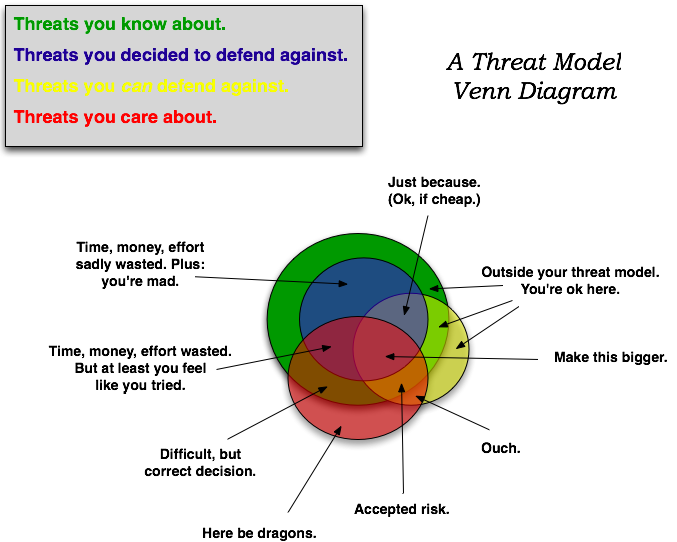
\includegraphics[scale=0.57]{pics/threat-model.eps} \\
\vspace{.2in}
\small
	\verb+https://www.netmeister.org/blog/threat-model-101.html.html+
\end{center}
\Normalsize
\vspace*{\fill}

\subsection{Threat Model}
\vspace*{\fill}
\begin{center}
	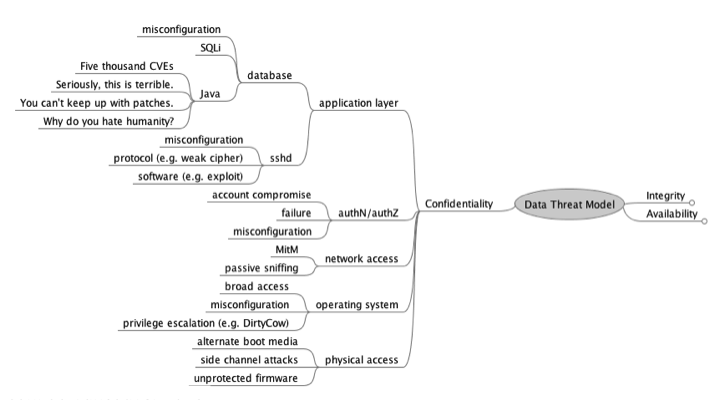
\includegraphics[scale=0.75]{pics/threat-model2.eps} \\
\vspace{.2in}
\small
	\verb+https://www.netmeister.org/blog/threat-model-101.html.html+
\end{center}
\Normalsize
\vspace*{\fill}



\subsection{Imperatives}
\vspace*{\fill}
\Huge
\begin{center}
Constantly seek to reduce your attack surface. \\
Identify and eliminate attack vectors.\\

\addvspace{.5in}
You can't do this alone:\\
lead by example, seek allies.
\end{center}
\Normalsize
\vspace*{\fill}

\subsection{Imperatives}
\vspace*{\fill}
\Huge
\begin{center}
{\em Never} think you're the only one who understands
or cares about security. \\

\addvspace{.5in}
{\em Always} consult with subject matter experts,
especially those {\em not} on your team.
\end{center}
\Normalsize
\vspace*{\fill}

\subsection{Defense in Depth}
\vspace*{\fill}
\Huge
\begin{center}
	Security is like an onion:
	the more layers you peel away, the more it stinks. \\
\addvspace{.5in}
\Normalsize
{\em Never} assume any one protection mechanism is sufficient. \\
\addvspace{.25in}
{\em Always} assume the other protections you deployed
can be circumvented or broken.
\end{center}
\vspace*{\fill}

\subsection{The biggest threat comes from the inside}
\vspace*{\fill}
\begin{center}
	
\includegraphics[scale=1.0]{pics/kane.eps} \\
\small
	{\em Never} ignore quarantine regulations.
\Normalsize
\end{center}
\vspace*{\fill}

\subsection{The biggest threat comes from the inside}
\vspace*{\fill}
\begin{center}
	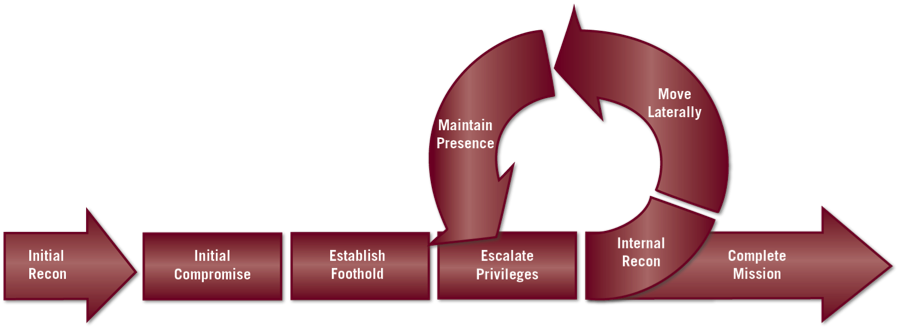
\includegraphics[scale=1.0]{pics/Killchain.eps} \\
\small
	\verb+http://is.gd/6sREQh+ \\
	\verb+https://www.netmeister.org/blog/attack-life-cycle.html+
\Normalsize
\end{center}
\vspace*{\fill}

\subsection{Cryptography}
\Normalsize
{\em Cryptography} can help mitigate {\em some} of the risks {\em sometimes}.

\subsection{Cryptography}
{\em Cryptography} can help mitigate {\em some} of the risks {\em sometimes}.
\\

It may provide security in the areas of:
\begin{itemize}
	\item Secrecy or Confidentiality
		\begin{itemize}
			\item {\em Did/could anybody else see (parts of) the message?}
		\end{itemize}
\end{itemize}

\subsection{Cryptography}
{\em Cryptography} can help mitigate {\em some} of the risks {\em sometimes}.
\\

It may provide security in the areas of:
\begin{itemize}
	\item Secrecy or Confidentiality
		\begin{itemize}
			\item {\em Did/could anybody else see (parts of) the message?}
		\end{itemize}
	\item Accuracy or Integrity
		\begin{itemize}
			\item {\em Was the message (could it have been) modified before I received it?}
		\end{itemize}
\end{itemize}

\subsection{Cryptography}
{\em Cryptography} can help mitigate {\em some} of the risks {\em sometimes}.
\\

It may provide security in the areas of:
\begin{itemize}
	\item Secrecy or Confidentiality
		\begin{itemize}
			\item {\em Did/could anybody else see (parts of) the message?}
		\end{itemize}
	\item Accuracy or Integrity
		\begin{itemize}
			\item {\em Was the message (could it have been) modified before I received it?}
		\end{itemize}
	\item Authenticity
		\begin{itemize}
			\item {\em Is the party I'm talking to actually
who I think it is / they claim they are?}
		\end{itemize}
\end{itemize}

\subsection{Cryptography}
Note:
\begin{itemize}
	\item {\em Never} write your own crypto or invent your own protocol.
	\item {\em Authentication} \verb+!=+ {\em Authorization}
	\item cryptography does not handle authorization
	\item you generally need all three: confidentiality, integrity, authenticity
	\item cryptography cannot prevent against incorrect use \\
		-- usability is hard!
\end{itemize}
\addvspace{.5in}
Know your threat model!

\subsection{Basic Security Concepts: Confidentiality}
\begin{itemize}
	\item Alice and Bob agree on a way to transform plain text into ciphertext
	\item transformed data is sent over insecure channel
	\item Alice and Bob are able to reverse transformation
\end{itemize}
\addvspace{.5in}
Different approaches:
\begin{itemize}
	\item secret key cryptography (example: {\em DES})
		\begin{itemize}
			\item Alice and Bob share a secret key (e.g. WEP, WPA−PSK, ...)
		\end{itemize}
\end{itemize}
\addvspace{.25in}
\begin{itemize}
	\item public key cryptography (example: {\em RSA})
		\begin{itemize}
			\item Alice has a private and a public key (e.g. TLS, SSH, PGP, ...)
			\item data encrypted with her private key can only be decrypted by
				her public key and vice versa
			\item public key can be shared with anybody (via insecure means)
		\end{itemize}
\end{itemize}

\subsection{Threats to Confidentiality}
\begin{itemize}
	\item lack of {\em authenticity}
	\item key exchange
	\item lack of key rotation
	\item key disclosure
\end{itemize}
\addvspace{.5in}
{\em Never} store secrets in code! \\
{\em Always} use a key management system.

\subsection{Basic Security Concepts: Integrity}
In order to protect against forgery or data manipulation, provide some sort of
digest or checksum (often a one-way hash).  Popular choices:

\begin{itemize}
	\item {\tt 5f4dcc3b5aa765d61d8327deb882cf99} (MD5)
	\item {\tt 5baa61e4c9b93f3f0682250b6cf8331b7ee68fd8} (SHA-1)
	\item {\tt 5e884898da28047151d0e56f8dc6292773603d0d6aabbdd62 \
                   a11ef721d1542d8} (SHA256)
	\item {\tt b109f3bbbc244eb82441917ed06d618b9008dd09b3befd1b5 \
                   e07394c706a8bb980b1d7785e5976ec049b46df5f1326af5a \
                   2ea6d103fd07c95385ffab0cacbc86} (SHA512)
\end{itemize}

\subsection{Basic Security Concepts: Integrity}
Examples: host based IDS, package manager signatures

\vspace{.5in}
Some possible threats:
\begin{itemize}
	\item collisions in algorithm
	\item lack of {\em authenticity} (Where did I get the checksum?)
	\item lack of {\em integrity} (Was the checksum tampered to match the (tampered) data?)
	\item ``verification'' with compromised tools
	\item ``rainbow tables'' / internet search engines allow for easy reverse
		lookup of un-salted hashes.
\end{itemize}

\subsection{Basic Security Concepts: Hashing Passwords}
{\em Never} confuse {\em hashing} and {\em encryption}! \\

{\em Never} encrypt your users' passwords to store them -- {\em always} hash them. \\

\addvspace{.25in}
{\em Always} salt your hashes. \\

{\em Always} use adaptive or key-stretching functions
such as e.g. {\tt bcrypt}, {\tt PBKDF2}, {\tt Argon2}.

\subsection{Basic Security Concepts: Authenticity}
Three general ways of proving that you are who you say you are:
\begin{itemize}
	\item something you know
	\item something you have
	\item something you are
\end{itemize}

\subsection{Basic Security Concepts: Authenticity}
Three general ways of proving that you are who you say you are:
\begin{itemize}
	\item something you know
		\begin{itemize}
			\item secret handshake, password
			\item can (easily) be given to and used by somebody else
		\end{itemize}
	\item something you have
	\item something you are
\end{itemize}

\subsection{Basic Security Concepts: Authenticity}
\begin{verbatim}
NetBSD/amd64 (SERVER) (console)

login: jschauma
password: *********************************
NetBSD 7.0.2 (SERVER) #2: Tue Jan 24 02:33:13 EST 2017

Welcome to NetBSD!
hostname$ 
\end{verbatim}

\subsection{Basic Security Concepts: Authenticity}
Three general ways of proving that you are who you say you are:
\begin{itemize}
	\item something you know
		\begin{itemize}
			\item secret handshake, password
			\item can (easily) be given to and used by somebody else
		\end{itemize}
	\item something you have
		\begin{itemize}
			\item physical items: smart card, RSA token, ...
			\item private keys
			\item can (easily) be given to and used by somebody else
		\end{itemize}
	\item something you are
\end{itemize}

\subsection{Basic Security Concepts: Authenticity}
\begin{verbatim}
$ ssh-keygen -l -f /dev/stdin <<<$(aws ec2 get-console-output \
        i-0990f1eb069c853c4 | grep ^ecdsa)
256 19:af:35:01:0b:2a:ee:3d:30:0f:69:11:cc:55:7c:20 (ECDSA)
$ ssh -i ~/.ssh/myawskey ec2-54-227-16-184.compute-1.amazonaws.com
The authenticity of host 'ec2-54-227-16-184.compute-1.amazonaws.com
(54.227.16.184)' can't be established.
ECDSA key fingerprint is 19:af:35:01:0b:2a:ee:3d:30:0f:69:11:cc:55:7c:20.
Are you sure you want to continue connecting (yes/no)?  yes
NetBSD 7.0.2 (SERVER) #2: Tue Jan 24 02:33:13 EST 2017

Welcome to NetBSD!
hostname$ 
\end{verbatim}

\subsection{Basic Security Concepts: Authenticity}
Three general ways of proving that you are who you say you are:
\begin{itemize}
	\item something you know
		\begin{itemize}
			\item secret handshake, password
			\item can (easily) be given to and used by somebody else
		\end{itemize}
	\item something you have
		\begin{itemize}
			\item physical items: smart card, RSA token, ...
			\item private keys
			\item can (easily) be given to and used by somebody else
		\end{itemize}
	\item something you are
		\begin{itemize}
			\item physical, physiological or behavioral traits
			\item cannot (easily or at all) be given to or
				used by somebody else
			\item cannot (easily or at all) be changed once
				compromised
		\end{itemize}
\end{itemize}

\subsection{Basic Security Concepts: Authenticity}
\vfill
\begin{center}
	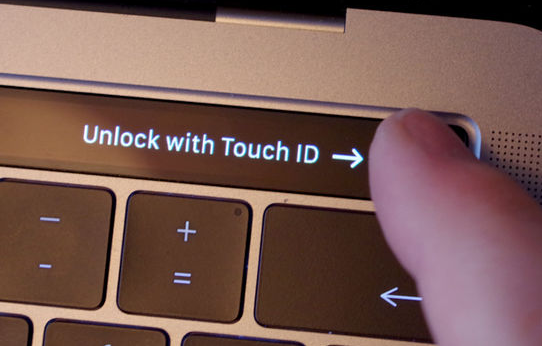
\includegraphics[scale=1.0]{pics/touchid.eps}
\end{center}
\vfill

\subsection{Basic Security Concepts: Authenticity}
Some possible threats:
\begin{itemize}
	\item lack of {\em confidentiality}
	\item lack of {\em integrity}
	\item reliance on fragile infrastructure
	\item usability
	\item conflation with {\em authorization}
\end{itemize}

\subsection{Principle of Least Privilege}
\vspace*{\fill}
\begin{center}
	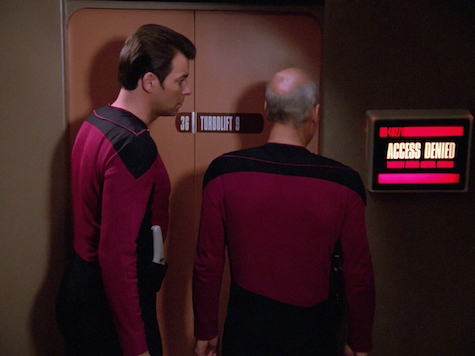
\includegraphics[scale=0.9]{pics/turbolift_access_denied.eps}
\end{center}
\vspace*{\fill}

\subsection{Principle of Least Privilege}

{\em Never} run services as root; {\em always} use a
dedicated account. \\

{\em Never} log in as root; {\em always} use {\tt
sudo(1)}. \\

{\em Never} rely on implicit privileges; {\em always}
grant access explicitly. \\

{\em Never} grant permanent overly broad access; {\em
always} use periodic access renewal and Role Based
Access Controls (RBAC).


\subsection{It's not just 1s and 0s}
\vspace{.5in}
\Huge
\begin{center}
System security is not restricted to {\em software} security.
\end{center}
\Normalsize

\subsection{It's not just 1s and 0s}
\vspace{.5in}
\Huge
\begin{center}
The thing that makes security difficult is not the software or hardware
components.  It's the human component.
\end{center}
\Normalsize

\subsection{It's not just 1s and 0s}
\vspace*{\fill}
\begin{center}
	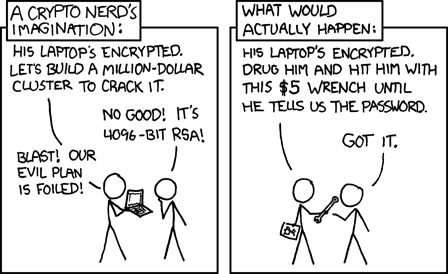
\includegraphics[scale=1.3]{pics/security.eps}
\end{center}
\vspace*{\fill}



\subsection{Secure by default}
\vspace{.5in}
\Huge
\begin{center}
Users care about usability, not about security.
\end{center}
\Normalsize

\subsection{Secure by default}
\vspace{.5in}
\Huge
\begin{center}
Users will not change their default settings.
\end{center}
\Normalsize

\subsection{Secure by default}
\vspace{.5in}
\Huge
\begin{center}
Users will not change their default settings. \\
\Normalsize
(Unless a less secure option is available.)
\end{center}

\newpage
\vspace*{\fill}
\begin{center}
    \Hugesize
        Hooray! \\ [1em]
    \hspace*{5mm}
    \blueline\\
    \hspace*{5mm}\\
        5 Minute Break
\end{center}
\vspace*{\fill}

\subsection{Classes of Vulnerabilities}
\Normalsize
\begin{itemize}
	\item memory management
		\begin{itemize}
			\item use of uninitialized memory
			\item buffer overflow / stack smashing
			\item use-after-free / dangling pointer
		\end{itemize}
	\item input validation
		\begin{itemize}
			\item code and command injections
			\item format attacks
			\item Little Bobby Tables ({\tt https://www.xkcd.com/327/})
		\end{itemize}
	\item race contitions
		\begin{itemize}
			\item non-atomic TOCTOU
			\item symlink attacks
		\end{itemize}
\end{itemize}

\subsection{Classes of Vulnerabilities}
\begin{itemize}
	\item privilege escalation and confusion
		\begin{itemize}
			\item XSS, CSRF
			\item setuid with untrusted environment
		\end{itemize}
	\item social engineering
		\begin{itemize}
			\item phishing
			\item watering hole attacks
		\end{itemize}
	\item brute-force attacks
		\begin{itemize}
			\item namespace iteration
			\item denial of service
		\end{itemize}
	\item information disclosure
		\begin{itemize}
			\item MitM
			\item insufficient permissions
			\item lack of encryption, authN, authZ
		\end{itemize}
\end{itemize}

\subsection{Security Fallacies and Pitfalls}
\vspace*{\fill}
\begin{center}
	\Hugesize
        Security by Obscurity \\
\end{center}
\vspace*{\fill}

\subsection{Security Fallacies and Pitfalls}
\vspace*{\fill}
\begin{center}
	\Hugesize
	Know what you're doing. \\
\addvspace{.25in}
	\Normalsize
	{\em Never} blindly apply nor dismiss a security mechanism. \\
\addvspace{.125in}
	{\em Always} know which threat you're mitigating.
\end{center}
\vspace*{\fill}

\subsection{Security Fallacies and Pitfalls}
\vspace*{\fill}
\begin{center}
    \Hugesize
        Perfect is the Enemy of the Good \\
	\vspace{.25in}
	\Normalsize
	(Differentiate between futile efforts and raising the bar.)
\end{center}
\vspace*{\fill}

\subsection{Security Fallacies and Pitfalls}
\vspace*{\fill}
\begin{center}
    \Hugesize
        One in a million is next Tuesday. \\
	\vspace{.25in}
	\Normalsize
	\verb+http://is.gd/Isb20K+
\end{center}
\vspace*{\fill}

\subsection{Security Fallacies and Pitfalls}
\vspace*{\fill}
\begin{center}
    \Hugesize
        ``Any person can invent a security system so clever that she or he
can't think of how to break it.'' \\
	\vspace{.25in}
	\Normalsize
	Schneier's Law \verb+http://is.gd/hW82dt+
\end{center}
\vspace*{\fill}

\subsection{Security Fallacies and Pitfalls}
\vspace*{\fill}
\begin{center}
    \Hugesize
        Don't invent your own crypto. \\
	\vspace{.25in}
	\Normalsize
	(Seriously, don't.)
\end{center}
\vspace*{\fill}

\subsection{Security Fallacies and Pitfalls}
\vspace*{\fill}
\begin{center}
    \Hugesize
	Complexity is the worst enemy of security. \\
	\vspace{.25in}
	\Normalsize
	(The more secure you make something, the less secure it becomes.)
\end{center}
\vspace*{\fill}

\subsection{Whom do you trust?}
\vspace*{\fill}
\begin{center}
\Huge
	Reflections on Trusting Trust \\

\Normalsize
	\verb+https://is.gd/RUX4zY+
\end{center}
\vspace*{\fill}
\Normalsize

\subsection{Outsourcing Services}
\begin{itemize}
	\item you trust the provider/vendor to honor the agreement
	\item you ``hope'' they won't change their agreement (once
		invested, changing back is hard)
	\item you trust the provider/vendor to keep their infrastructure
		safe
	\item you trust the provider/vendor's employees
	\item you are ok with the traffic going across the public internet
\end{itemize}

\subsection{Outsourcing Services}
\begin{itemize}
	\item you trust the provider/vendor to honor the agreement
	\item you ``hope'' they won't change their agreement (once
		invested, changing back is hard)
	\item you trust the provider/vendor to keep their infrastructure
		safe
	\item you trust the provider/vendor's employees
	\item you are ok with the traffic going across the public internet
\end{itemize}
\addvspace{.5in}
Bottom-line: are you increasing or decreasing your
attack surface? \\

\addvspace{.25in}
{\em Always} make a conscious decision; {\em never} blindly follow
the promises without understanding the trade-offs.

\subsection{Embrace Automation}
\vspace*{\fill}
\Huge
\begin{center}
	Vulnerabilities are dense. \\
\addvspace{.5in}
	Eliminate {\em classes} of attacks, not
	individual flaws. \\
\end{center}
\Normalsize
\vspace*{\fill}

\subsection{Build Robust Infrastructures and Service}
\vspace*{\fill}
\Huge
\begin{center}
	Your endpoint security model should assume the
	network is compromised; \\
	your network security model should assume the
	endpoint is. \\
\addvspace{.5in}
	Both in fact are.
\end{center}
\Normalsize
\vspace*{\fill}

\subsection{Toning down the Paranoia}
\vspace*{\fill}
\begin{center}
    \Hugesize
        Proving a Negative \\
	\vspace{.25in}
	\Normalsize
	(Evidence of Absences vs. Absence of Evidence)
\end{center}
\vspace*{\fill}


\subsection{Toning down the Paranoia}
\vspace*{\fill}
\Huge
\begin{center}
Never attribute to malice that which can be adequately explained by stupidity. \\
\vspace{.25in}
\Normalsize
Hanlon's Razor
\end{center}
\Normalsize
\vspace*{\fill}

\subsection{Toning down the Paranoia}
\vspace*{\fill}
\Huge
\begin{center}
Know which threat you're facing. \\
\vspace{.25in}
Know which mechanisms can help you. \\
Don't dismiss those.
\end{center}
\Normalsize
\vspace*{\fill}



\subsection{Sysadmin $\cap$ Infosec}
\vspace*{\fill}
\begin{center}
	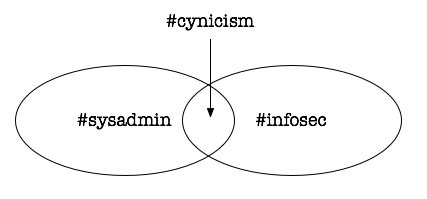
\includegraphics[scale=1.0]{pics/sysadmin_infosec.eps} \\
	\verb+https://www.netmeister.org/blog/infosec-basics.html+
\end{center}
\vspace*{\fill}

\subsection{Sysadmin $\cap$ Infosec}
\vspace*{\fill}
\Huge
\begin{center}
	Nothing is always absolutely so.
\end{center}
\Normalsize
\vspace*{\fill}

\subsection{Two Questions}
\vspace*{\fill}
\begin{center}
	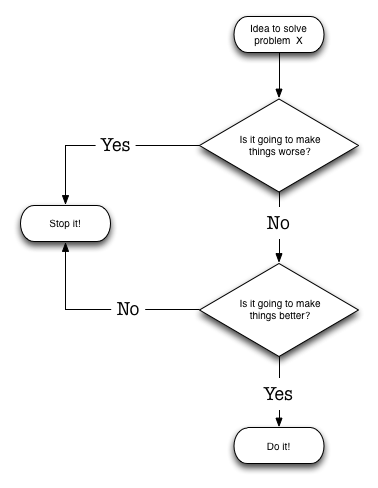
\includegraphics[scale=0.67]{pics/two-questions.eps} \\
\small
	\verb+https://www.netmeister.org/blog/two-questions.html+
\end{center}
\Normalsize
\vspace*{\fill}

\subsection{Last Words of Advice}
\begin{itemize}
	\item keep your asset inventory accurate
	\item don't shell out; parametrize arguments and {\tt exec(3)}
	\item don't trust the environment
	\item use multi-factor authentication
	\item use a password manager
	\item use a key management system
	\item rotate your secrets frequently
	\item {\tt curl -k} is a (contagious) symptom
	\item don't MitM your own users
	\item disable Flash; use an ad-blocker
	\item sign your software, configs; verify all signatures
	\item ensure secure defaults (e.g. umask, shell history, ...)
\end{itemize}

\subsection{Infosec Foundation}
\vspace*{\fill}
\Huge
\begin{center}
	Don't be lazy.
\end{center}
\Normalsize
\vspace*{\fill}

\subsection{Final Project}
Group project: Capture the Flag \\

\vspace{.5in}
\begin{verbatim}
https://www.cs.stevens.edu/~jschauma/615/ctf.html
\end{verbatim}

\subsection{Additional Reading}
\begin{verbatim}
https://www.slideshare.net/zanelackey/attackdriven-defense
https://www.netmeister.org/blog/moving-the-needle.html
https://www.netmeister.org/blog/attack-life-cycle.html
https://www.netmeister.org/blog/threat-model-101.html
https://twitter.com/jschauma/status/713118376550404096
https://t.co/DRHbEKXod8
https://danielmiessler.com/study/security_and_obscurity/
https://is.gd/sGnRVL
\end{verbatim}


\end{document}
